\documentclass{standalone}
\usepackage{tikz}
\usetikzlibrary{positioning,shapes.symbols}
%
\begin{document}

\begin{tikzpicture}
  \node[anchor=south west,inner sep=0] (image) at (0,0) {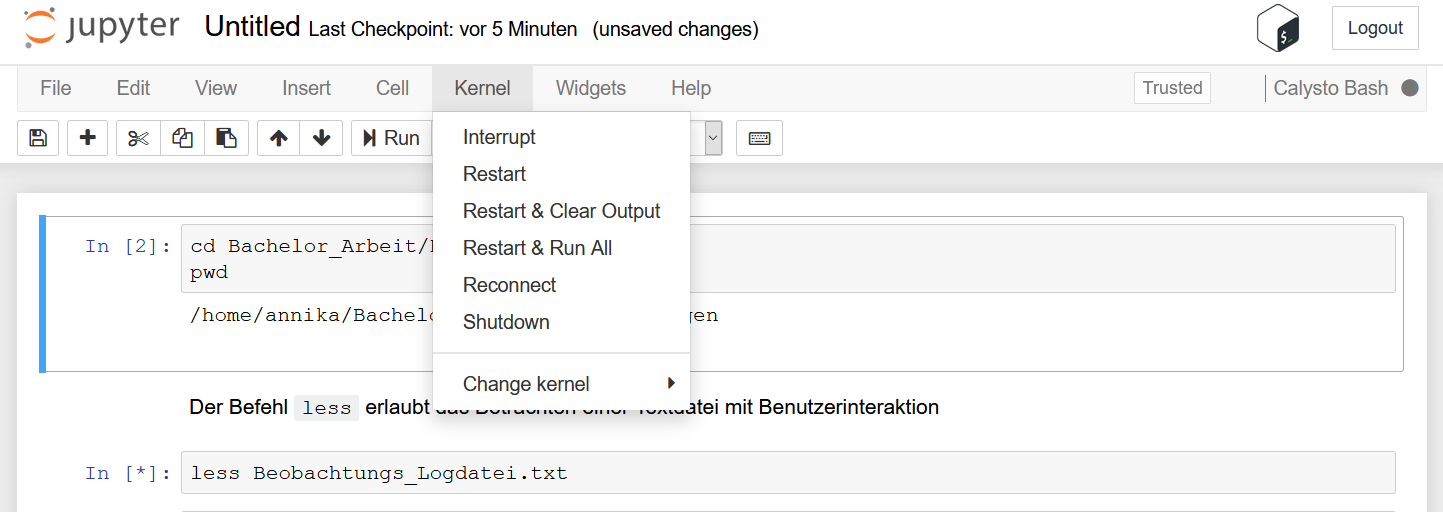
\includegraphics[width=5cm]{figuren/Restart_Kernel}};
  %
  \begin{scope}[x={(image.south east)},y={(image.north west)}]
    %\draw[help lines, very thin, step=0.02] (0,0) grid (1,1);
    %\draw[help lines,thin,xstep=.1,ystep=.1] (0,0) grid (1,1);
    %\foreach \x in {0,1,...,9} { \node [anchor=north] at (\x/10,0) {0.\x}; }
    %\foreach \y in {0,1,...,9} { \node [anchor=east] at (0,\y/10) {0.\y}; }
    \node[fill = green!10, font=\tiny, align = center] (ok) at (0.08, 1.1) {ok};
    \node[fill = blue!10, font=\tiny, align = center] (Problem) at (0.3, 1.1) {Problem};
    \node[fill = red!10, font=\tiny, align = center] (Kernel) at (0.63, 1.1) {Kernel \\ neu starten};
    \draw[red, thick] (0.31, 0.55) rectangle (0.47, 0.62);
    \draw[blue, thick] (0.05, 0.04) rectangle (0.13, 0.12);
    \draw[black!30!green, thick] (0.05, 0.48) rectangle (0.13, 0.56);
    \draw[-latex, black!30!green, thick] (ok) to (0.08, 0.56);
    \draw[-latex, blue, thick] (Problem) to (0.08, 0.12);
    \draw[-latex, red, thick] (Kernel) to (0.39, 0.62);
  \end{scope}
\end{tikzpicture}

\end{document}
